% Created 2015-11-06 Fri 17:51
\documentclass[a5paper]{book}
\usepackage[utf8]{inputenc}
\usepackage[T1]{fontenc}
\usepackage{fixltx2e}
\usepackage{graphicx}
\usepackage{grffile}
\usepackage{longtable}
\usepackage{wrapfig}
\usepackage{rotating}
\usepackage[normalem]{ulem}
\usepackage{amsmath}
\usepackage{textcomp}
\usepackage{amssymb}
\usepackage{capt-of}
\usepackage{hyperref}
\usepackage[unicode,dvipdfm]{hyperref}
\usepackage{fontspec}
\usepackage{xeCJK}
\setCJKmainfont{SimSun}
\setcounter{secnumdepth}{3}
\author{Jichao Ouyang}
\date{\textit{<2015-05-13 Wed>}}
\title{Functional JavaScript Mini Book}
\hypersetup{
 pdfauthor={Jichao Ouyang},
 pdftitle={Functional JavaScript Mini Book},
 pdfkeywords={},
 pdfsubject={},
 pdfcreator={Emacs 24.5.1 (Org mode 8.3.2)}, 
 pdflang={English}}
\begin{document}

\maketitle
\tableofcontents

\begin{quote}
如果你觉得这本书对你有帮助,忍不住要请\href{https://gum.co/fpjs}{我一杯咖啡}, 那么你将同时获得一本pdf版本的FPJS mini nook
\end{quote}

\part{Preface}
\label{sec:orgheadline1}
这是本可能2小时就能看完的小书,但是涵盖了基本所有函数式编程的内容,还包含了一些
ECMAScript 6 定义的函数式新特性, 如箭头函数, 模式匹配等等.
还会介绍函数式一些重要概念在 JavaScript是如何实现即应用,
以及如何以函数式的思想编写 JavaScript 代码.

\begin{quote}
本书虽然与我翻译的Michael Fogus的\href{http://book.douban.com/subject/22733640/}{Functional JavaScript}同名, 但是请不要当成是Fogus大师的mini版本, 
这里的内容完全跟Fogus大师的不一样, 可能比大师的要再"函数式"一些\footnote{Fogus同时是The Joy of Clojure的作者,我
特别奇怪为什么不把Clojure真正Good part写进Functional JavaScript里}, 用js实现了一些其他函数式语言(Clojure, Haskell)特有的函数式features.
\end{quote}

对果JavaScript的基本概念对你来说:

\url{./images/preface/what_you_talking.gif}

可能本书并不适合你, 请先移步 \href{https://leanpub.com/javascript-allonge}{JavaScript Allonge},
但是如果你学习函数式编程时感到费解:

\url{./images/preface/summarize_in_one_word.gif}

那么这本书将会对你会有所帮助.

我选用的 JavaScript 函数式库是
\href{https://rawgit.com/CrossEye/eweda/master/docs/eweda.html}{Eweda}(\href{https://ramdajs.com}{Ramda} 的最初实现,更遵守函数式教条,但由于
javascript 的栈很容易爆,Ramda的实现要更 pratical
一些而且可以用的产品代码中, 千万不要在产品中用
eweda,这里只用eweda做介绍目的)

\begin{quote}
\href{http://fr.umio.us/why-ramda/}{为什么不用 Underscore/Lodash} 请移步第二章
\end{quote}

\begin{quote}
由于会介绍 ECMAScript 6 的新特性, 书中很多写法都是 ECMAScript
6 标准, 只能在实现这些 feature 的浏览器(如 Firefox,
请目前参照各浏览器的\href{http://kangax.github.io/compat-table/es6/}{实现情况}) 里运行.
另外, 大多数的例子源码都会在文章里的 jsbin 链接里.
\end{quote}

\part{Lambda}
\label{sec:orgheadline9}
为什么讲 lambda, 如果小时候玩过游戏"半条命",那么你早都见过 lambda 了.


\includegraphics[width=.9\linewidth]{./images/lambda/Lambda_reactor_complex_logo.png}

我从wikipedia里面粘出来了这么一段定义:
\begin{quote}
lambda包括一条变换规则(变量替换)和一条函数定义方式,Lambda演算之通用在于,任何一个可计算函数都能用这种形式来表达和求值。因而,它是等价于图灵机的.
\end{quote}

好吧, 跟没解释一样. 简单来说lambda其实就是 \texttt{x} 到 \texttt{y} 的映射关系, 但在大部分支持函数式的编程语言中,
它等价于匿名函数. 被称为 lambda 表达式.
因为这些函数只需要用一次, 而且变换不复杂, 完全不需要命名.

\url{./images/lambda/parallel-universe.gif}

匿名函数在程序中的作用是可以作为参数传给高阶函数\footnote{第二章会详细解释高阶函数和闭包.}, 或者作为闭包被返回.

但是匿名函数并不是原本的 lambda 算子, 因为匿名函数也可以接受多个参数, 如

\begin{verbatim}
multiple(x, y) = x*y
\end{verbatim}

写成简单映射的形式, 把名字去掉

\begin{verbatim}
(x,y) -> x*y
\end{verbatim}

这就是 lambda 了吗, 不是, lambda的用意是简化这个映射关系以至不需要名字,
更重要的是只映射一个 x.

什么意思呢? 让我们来分解一下上面的这个映射的过程.

\begin{enumerate}
\item lambda 接受第一个参数 \texttt{5}, 返回另一个 lambda

\begin{verbatim}
(5) -> (y -> 5*y)
\end{verbatim}

\item 该返回的 lambda \texttt{y -> 5*y} 接收 \texttt{y} 并且返回 \texttt{5*y}, 若在用 \texttt{4} 调用该 lambda
\end{enumerate}

\begin{verbatim}
es6 -> 5*4
\end{verbatim}

因此这里的匿名函数 \texttt{(x,y)->x*y} 看似一个 lambda, 其实是两个 lambda
的结合.

而这种接受一个参数返回另一个接收第二个参数的函数叫柯里化\footnote{柯里化会在第二章详细讨论.}.

这里我们先忍一忍, 来看下 JavaScript 中的 lambda 表达式.
\chapter{箭头函数(arrow function)}
\label{sec:orgheadline5}

来看看越来越函数式の JavaScript

新的草案\href{http://kangax.github.io/compat-table/es6/}{ECMAScript 6}
(虽然说是草案,但你可以看到 Firefox 其实已经实现大部分的
feature)里我们越来越近了, 借助一下transcompiler例如\href{https://babeljs.io}{Babel} 我们完全可以在项目中开始使用es6了\footnote{可以看看es6比较有意思的新特性 \url{http://blog.oyanglul.us/javascript/essential-ecmascript6.html}}。

看看里面有一行 arrow
function,为什么叫箭头函数,还记得前面说lambda是提到的箭头吗。而且如果你之前用过
Haskell(单箭头) 或者Scala(双箭头), 会发现都用的是箭头来表示简单映射关系.

\begin{quote}
由于 arrow function 只在Firefox 22以上版本实现,
本节的所有代码都可以在Firefox的Console中调试, 其他chrome 什么的都没有实现(完全)\footnote{Chrome有一个 feature toggle 可以打开部分 es6 功能 \texttt{chrome://flags/\#enable-javascript-harmony}}.
另外每节的最后我都会给出完整代码的可执行的 jsbin 链接.
\end{quote}

\section{声明一个箭头函数}
\label{sec:orgheadline2}

你可以用两种方式定义一个箭头函数

\begin{verbatim}
([param] [, param]) => {
   statements
}
// or
param => expression
\end{verbatim}

单个表达式可以写成一行, 而多行语句则需要 block \texttt{\{\}} 括起来.

\section{为什么要用箭头函数}
\label{sec:orgheadline3}

看看旧的匿名函数怎么写一个使数组中数字都乘2的函数.

\begin{verbatim}
var a = [1,2,curry,es6,5];
a.map(function(x){ return x*2 });
\end{verbatim}

用箭头函数会变成

\begin{verbatim}
a.map(x => x*2);
\end{verbatim}

只是少了 \texttt{function} 和 \texttt{return} 以及 block, 不是吗? 如果觉得差不多,
因为你看惯了 JavaScript 的匿名函数,
你的大脑编译器自动的忽略了,因为他们不需要显示的存在.

而 \texttt{map(x => x*2)} 要更 make sense,
因为我们需要的匿名函数只需要做一件事情, 我们需要的是 一个函数 \texttt{f},
可以将给定 \texttt{x}, 映射到 \texttt{y}.
翻译这句话的最简单的方式不就是 \texttt{f = (x => x*2)}

\section{Lexical \texttt{this}}
\label{sec:orgheadline4}

如果你觉得这还不足以说服改变匿名函数的写法,
那么想想以前写匿名函数中的经常需要 \texttt{var self=this} 的苦恼.

\begin{verbatim}
    var Multipler = function(inc){
      this.inc = inc;
    }
    Multipler.prototype.multiple = function(numbers){
      return numbers.map(function(number){
        return this.inc * number;
      })
    }
    new Multipler(2).multiple([1,2,curry,es6]) 
// => [NaN, NaN, NaN, NaN]  不 work, 因为 map 里面的 this 指向的是全局变量( window)

    Multipler.prototype.multiple = function(numbers){
      var self = this; // 保持 Multipler 的 this 的缓存
      return numbers.map(function(number){
        return self.inc * number;
      })
    }
    new Multipler(2).multiple([1,2,curry,es6]) // => [ 2, es6, 6, 8 ]
\end{verbatim}

很怪不是吗, 确实是 Javascript 的一个 bug, 因此经常出现在各种面试题中, 问 \texttt{this} 到底是谁.

\url{./images/lambda/which-leela.gif}

试试替换成 arrow function

\begin{verbatim}
Multipler.prototype.multiple = function(numbers){
  return numbers.map((number) => number*this.inc);
};

console.log(new Multipler(2).multiple([1,2,curry,es6]));// => [ 2, es6, 6, 8 ]
\end{verbatim}

不需要 \texttt{var self=this} 了是不是很开心☺️现在, arrow function 里面的
this 会自动 capture 外层函数的 \texttt{this} 值.

\chapter{JavaScript的匿名函数(anonymous function)}
\label{sec:orgheadline8}

支持匿名函数, 也就意味着函数可以作为一等公民. 可以被当做参数,
也可以被当做返回值.因此, JavaScript 的支持一等函数的函数式语言,
而且定义一个匿名函数式如此简单.

\section{创建一个匿名函数}
\label{sec:orgheadline6}

在JavaScript里创建一个函数是如此的 \sout{简单} \ldots{} 比如:
\begin{verbatim}
function(x){
    return x*x;
}// => SyntaxError: function statement requires a name
\end{verbatim}

但是, 为什么报错了这里. 因为创建一个匿名函数需要用表达式(function
expression). 表达式是会返回值的:

\begin{verbatim}
var a = new Array() // new Array 是表达式, 而这整行叫语句 statement
\end{verbatim}

但为什么说 \texttt{function statement requires a name}. 因为 JavaScript
\textbf{还有一种} 创建函数的方法--/function statement/.
而在上面这种写法会被认为是一个 function 语句, 因为并没有期待值. 而
function 语句声明是需要名字的.

简单将这个函数赋给一个变量或当参数传都不会报错,
因为这时他没有歧义,只能是表达式.比如:

\begin{verbatim}
var squareA = function(x){
    return x*x;
}
\end{verbatim}

但是这里比较 tricky 的是这下 \texttt{squareA} 其实是一个具名函数了.

\begin{verbatim}
console.log(squareA) // => function squareA()
\end{verbatim}

虽然结果是具名函数,但是过程却与下面这种声明的方式不一样.

\begin{verbatim}
function squareB(x){
    return x*x;
} // => undefined
\end{verbatim}

\texttt{squareB} 用的是 function statement 直接声明(显然 statement 没有返回),
而 \texttt{squareA} 则是先用 function expression 创建一个匿名函数,
然后将返回的函数赋给了名为 \texttt{squareA} 的变量. 因为表达式是有返回的:

\begin{verbatim}
console.log(function(x){ return x*x});
// => undefined
// => function ()
\end{verbatim}

第一个 \texttt{undefined} 是 \texttt{console.log} 的返回值, 因此
\texttt{function()} 则是打印出来的 function 表达式创建的匿名函数.

\section{使用匿名函数}
\label{sec:orgheadline7}

JavaScript 的函数是一等函数. 这意味着我们的函数跟值的待遇是一样的,于是它

可以赋给变量:

\begin{verbatim}
var square = function(x) {return x*x}
\end{verbatim}

可以当参数, 如刚才见到的:

\begin{verbatim}
console.log(function(x){return x*x})
\end{verbatim}

将函数传给了 \texttt{console.log}

可以被返回:

\begin{verbatim}
function multiply(x){
    return function(y){
        return x*y;
    }
}
multiply(1)(2) // => 2
\end{verbatim}

\part{高阶函数(Higher-order function)}
\label{sec:orgheadline23}

我们已经见识到了匿名函数和箭头函数的用法, 匿名的一等函数到底有什么用呢?
来看看高阶函数的应用.

高阶函数意思是它接收另一个函数作为参数. 为什么叫 \textbf{高阶}: 来看看这个函数
\texttt{f(x, y) = x(y)} 按照 lambda 的简化过程则是

\begin{verbatim}
f(x) => (y -> x(y))
(y) => x(y)
\end{verbatim}

可以看出来调用 f 时却又返回了一个函数x.

还记得高等数学里面的导数吗, 两阶以上的导数叫高阶导数.
因为求导一次以后返回的可以求导.

概念是一样的,
如同\href{https://en.wikipedia.org/wiki/Matryoshka_doll}{俄罗斯套娃} 当函数执行以后还需执行或者要对参数执行,
因此叫高阶函数.


\includegraphics[width=.9\linewidth]{./images/higherorder/recursion.png}

高阶函数最常见的应用如 \texttt{map}, \texttt{reduce}.
他们都是以传入不同的函数来以不同的方式操作数组元素.

另外 \emph{柯里化}, 则是每次消费一个参数并返回一个逐步被配置好的函数.
\index{柯里化}
\index{currying}

高阶函数的这些应用都是为函数的组合提供灵活性.
在本章结束相信你会很好的体会到函数组合的强大之处.

\chapter{Higher-order function}
\label{sec:orgheadline12}

函数在 JavaScript 中是一等公民, 因此在 JavaScript 中, 使用高阶函数是非常方便的.

\section{函数作为参数}
\label{sec:orgheadline10}

假设我现在要对一个数组排序, 用我们熟悉的 \texttt{sort}

\begin{verbatim}
[1,3,2,5,4].sort( (x, y) => x - y )
\end{verbatim}

如果我们要逆序的排序, 把减号左右的 \texttt{x} 和 \texttt{y} 呼唤,就这么简单,
但如果我是一个对象数组, 要根据对象的 \texttt{id} 排序:

\begin{verbatim}
[{id:1, name:'one'},
 {id:3, name:'three'}, 
 {id:2, name:'two'}, 
 {id:5, name:'five'},  
 {id:4, name:'four'}].sort((x,y) => x.id - y.id)
\end{verbatim}

是不是已经能够感受到高阶函数与匿名函数组合的灵活性.

\section{函数作为返回值}
\label{sec:orgheadline11}

函数的返回值可以不只是值, 同样也可以是一个函数, 来看 Eweda
内部的一个工具函数 \texttt{aliasFor}, 他的作用是给函数 E 的一些方法起一些别名:

\begin{quote}
听起来很怪不是吗, 函数怎么有方法, 实际上 JavaScript 的 \texttt{function}
是一个特殊 \textbf{对象}, 试试在 Firefox console 里敲 \texttt{console.log.}
是不是看到了一些方法, 但是 \texttt{typeof console.log} 是 function
\end{quote}

\begin{verbatim}
var E = () => {}
var aliasFor = oldName => {
    var fn = newName => {
      E[newName] = E[oldName];
      return fn;
    };
    return (fn.is = fn.are = fn.and = fn);
};
\end{verbatim}

这里有两个 \texttt{return}, 一个是 \texttt{fn} 返回自己, 另一个是 \texttt{aliasFor} 也返回
\texttt{fn}, 并且给 \texttt{fn} 了几个别名 \texttt{fn.is} \texttt{fn.are}\ldots{}

什么意思呢? \texttt{fn} 返回 \texttt{fn}. 很简单就是 \texttt{fn() => fn},
那么 \texttt{fn()()=>fn()=>fn} \ldots{}以此类推, 无论调用 fn 多少次,都最终返回 fn.


\includegraphics[width=.9\linewidth]{./images/higherorder/1qUCC8s.png}

这到底有什么用呢, 由于这里使用了 \texttt{fn} 的副作用(side affect)
来干了一些事情 \texttt{E[newName]=E[oldName]}, 也就是给 E 的方法起一个别名,
因此每次调用 fn 都会给 \texttt{E} 起一个别名. \texttt{aliasFor} 最后返回的是 \texttt{fn}
自己的一些别名, 使得可以 chain 起来更可读一些:

\begin{verbatim}
aliasFor('reduce').is('reduceLeft').is('foldl')
\end{verbatim}

\begin{quote}
另外, 函数作为返回值的重要应用, 柯里化与闭包,
将会在在后面专门介绍. 我们先来看下以函数作为参数的高阶函数的典型应用.
\end{quote}

\chapter{柯里化 currying}
\label{sec:orgheadline19}

还记得 Haskell Curry吗


\includegraphics[width=.9\linewidth]{./images/higherorder/curry.png}

多巧啊, 人家姓 Curry 名 Haskell, 难怪 Haskell 语言会自动柯里化, 呵呵.
但是不奇怪吗, 为什么要柯里化呢. 为什么如此重要得让 Haskell
会默认自动柯里化所有函数, 不就是返回一个部分配置好的函数吗.

我们来看一个 Haskell 的代码.

\begin{verbatim}
max 3 4
(max 3) 4
\end{verbatim}

结果都是4, 这有什么用呢.

这里看不出来, 放到 \texttt{高阶函数} 试试. 什么? 看不懂天书 Haskell, 来看看
JavaScript 吧.

\section{我们来看一个问题}
\label{sec:orgheadline16}

\begin{itemize}
\item 写一个函数, 可以连接字符数组, 如 f(['1','2']) => '12'
\label{sec:orgheadline13}

好吧,如果不用柯里化, 怎么写? 啊哈 \texttt{reduce}

\begin{verbatim}
var concatArray = function(chars){
  return chars.reduce(function(a, b){
    return a.concat(b);
  });
}
concat(['1','2','3']) // => '123'
\end{verbatim}

很简单,对吧.

\item 现在我要其中所有数字加1, 然后在连接
\label{sec:orgheadline14}

\begin{verbatim}
var concatArray = function(chars, inc){
  return chars.map(function(char){
    return (+char)+inc + '';
  }).reduce(function(a,b){
      return a.concat(b)
  });
}
console.log(concatArray(['1','2','3'], 1))// => '234'
\end{verbatim}

\item 所有数字乘以2, 再重构试试看
\label{sec:orgheadline15}

\begin{verbatim}
var multiple = function(a, b){
  return +a*b + ''
}
var concatArray = function(chars, inc){
  return chars.map(function(char){
    return multiple(char, inc);
  }).reduce(function(a,b){
      return a.concat(b)
  });
}
console.log(concatArray(['1','2','3'], 2)) // => '246'
\end{verbatim}

是不是已经看出问题了呢?
如果我在需要每个数字都减2,是不是很麻烦呢.需要将 \texttt{map} 参数匿名函数中的
multiple 函数换掉. 这样一来 \texttt{concatArray} 就不能同时处理加, 乘和减?
那么怎么能把他提取出来呢? 来对比下柯里化的解法.
\end{itemize}

\section{柯里化函数接口}
\label{sec:orgheadline17}

\begin{verbatim}
var multiple = function(a){
  return function(b){
    return +b*a + ''
  }
}

var plus = function(a){
  return function(b){
    return (+b)+a + ''
  }
}
var concatArray = function(chars, stylishChar){
  return chars.map(stylishChar)
    .reduce(function(a,b){
      return a.concat(b)
  });
}
console.log(concatArray(['1','2','3'], multiple(2)))
console.log(concatArray(['1','2','3'], plus(2)))
\end{verbatim}

有什么不一样呢 1. 处理数组中字符的函数被提取出来, 作为参数传入 2.
提取成柯里化的函数, 部分配置好后传入, 好处显而易见, 这下接口非常通畅
无论是外层调用

\begin{verbatim}
concatArray(['1','2','3'], multiple(2))
\end{verbatim}

还是内部的 map 函数

\begin{verbatim}
chars.map(stylishChar)
\end{verbatim}

这些接口都清晰了很多, 不是吗

这就是函数式的思想, 用已有的函数组合出新的函数, 而柯里化每消费一个参数,
都会返回一个新的部分配置的函数, 这为函数组合提供了更灵活的手段,
并且使得接口更为流畅.

\section{自动柯里化}
\label{sec:orgheadline18}

在 Haskell 语言中, 函数是会自动柯里化的:

\begin{verbatim}
max 3 4
\end{verbatim}

其实就是

\begin{verbatim}
(max 3) 4
\end{verbatim}

可以看看 \texttt{max} 与 \texttt{max 3} 函数的 类型

\begin{verbatim}
ghci> :t max
max :: Ord a => a -> a -> a
\end{verbatim}

看明白了么, \texttt{Ord a =>} 表示类型约束为可以比较大小的类型, 因此 \texttt{max}
的类型可以翻译成: 当给定一个 \texttt{a}, 会得到 \texttt{a -> a},
再看看 \texttt{max 3} 的类型就好理解了

\begin{verbatim}
ghci> :t max 3
(Num a, Ord a) => a -> a
\end{verbatim}

左侧表示类型约束 \texttt{a} 可以是 \texttt{Ord} 或者 \texttt{Num},
意思是 \texttt{max 3} 还是一个函数,如果给定一个 \texttt{Ord} 或者 \texttt{Num} 类型的参数
则返回一个 \texttt{Ord} 或者 \texttt{Num}.

现在是不是清晰了, 在 Haskell 中每给定一个参数, 函数如果是多参数的,
该函数还会返回一个处理余下参数的函数. 这就是自动柯里化.

而在 Javascript(以及大多数语言) 中不是的, 如果给定多参函数的部分参数,
函数会默认其他参数是 \texttt{undefined}, 而不会返回处理剩余参数的函数.

\begin{verbatim}
function willNotCurry(a, b, c) {
    console.log(a, b, c)
    return a*b-c;
}
willNotCurry(1)
// => NaN
// => 1 undefined undefined
\end{verbatim}

如果使用自动柯里化的库 \href{https://github.com/CrossEye/eweda}{eweda},
前面的例子简直就完美了

\begin{verbatim}
var multiple = curry(function(a, b){
  return +b*a + ''
})
var plus = curry(function(a, b){
  return (+b)+a + ''
})
\end{verbatim}

\chapter{函数组合 function composition}
\label{sec:orgheadline22}

通过前面介绍的高阶函数, map, fold 以及柯里化,
其实已经见识到什么是函数组合了. 如之前例子中的 map 就是 由 fold 函数与
reverse 函数组合出来的.

这就是函数式的思想, 不断地用已有函数, 来组合出新的函数.

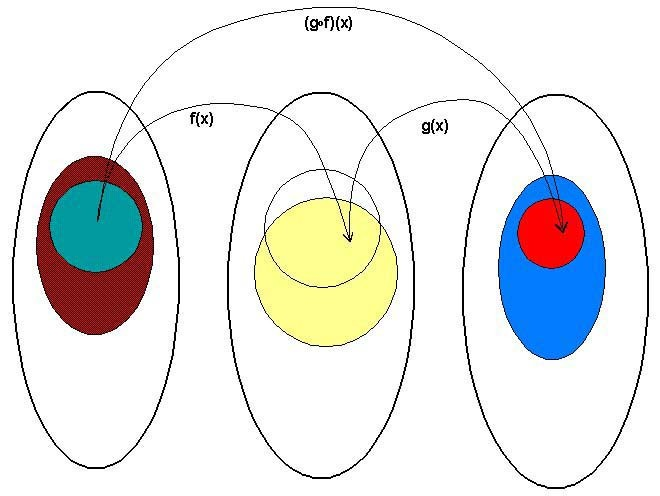
\includegraphics[width=.9\linewidth]{./images/higherorder/composition.jpg}

如图就是函数组合,来自
\href{https://en.wikipedia.org/wiki/Category_theory}{Catgory Theory}(Funtor 也是从这来的,后面会讲到), 既然从 A到B
有对应的映射f,B到 C有对应的映射g, 那么 \texttt{(g.f)(x)} 也就是 \texttt{f} 与 \texttt{g}
的组合 \texttt{g(f(x))} 就是 A到 C 的映射。上一章实现的 map 函数就相当于
\texttt{reverse.fold}.

\section{Compose}
\label{sec:orgheadline20}

我们可以用 Eweda 非常方便的 compose 方法来组合函数

\begin{verbatim}
var gf = E.compose(f, g)
\end{verbatim}

说到了函数组合, 柯里化, 我想现在终于可以解释清楚为什么在这里选用
Eweda/Ramda 而不是 Underscore 了.

举个例子🌰 如果我现在想要 tasks 列表中所有属性为 \texttt{completed} 为 \texttt{true}
的元素, 并按照 \texttt{id} 排序.

underscore 里会这样写:

\begin{verbatim}
_(tasks)
    .chain()
    .filter( task => task.completed===true)
    .sortBy( task => task.id)
    .value();
\end{verbatim}

这种方式怎么看都不是函数式, 而是以对象/容器为中心的串联,有些像 jquery
对象的链式调用, 或者我们可以写的函数式一些, 如

\begin{verbatim}
_.sortBy(_.filter(tasks, task => task.completed===true), task => task.id)
\end{verbatim}

恩恩, 看起来不错嘛, 但是有谁是这么用 underscore的呢. 一般都会只见过
链式调用才是 underscore 的标准写法。

来对比一下用 Eweda/Ramda 解决的过程 :

\begin{verbatim}
compose(sortBy(task=>task.id), filter(task=>task.completed===true))(tasks)
\end{verbatim}

好像没什么区别啊? 不就是用了 compose 吗?

区别大了这, 看见 \texttt{tasks} 是最后当参数传给 \texttt{E.compose()} 的吗?
而不是写死在filter 的参数中. 这意味着在接到需要处理的数据前,
我已经组合好一个新的函数在等待数据, 而不是把数据混杂在中间,
或是保持在一个中间对象中. 而 underscore
的写法导致这一长串 \texttt{\_.sortBy(\_.filter())} 其实根本无法重用。

好吧如果你还看不出来这样做的好处. 那么来如果我有一个包含几组 tasks的列表
groupedTasks, 我要按类型选出 completed 为 true 并按 id 排序.
如我现在数据是这个:

\begin{verbatim}
groupedTasks = [
  [{completed:false, id:1},{completed:true, id:2}],
  [{completed:false, id:4},{completed:true, id:3}]
]
\end{verbatim}

underscore:

\begin{verbatim}
_.map(groupedTasks,
   tasks => _.sortBy(_.filter(tasks, task => task.completed===true), task => task.id))
\end{verbatim}

看见我们又把 \texttt{\_.sortBy(\_.filter())} 这一长串原封不动的拷贝到了 map 里。
因为 underscore
一开始就要消费数据,使得很难重用,除非在套在另一个函数里:

\begin{verbatim}
function completedAndSorted(tasks){
  return _.sortBy(_.filter(tasks, task => task.completed===true), task => task.id))
}
_.map(groupedTasks, completedAndSorted)
\end{verbatim}

只有这样才能重用已有的一些函数。或者虽然 underscore 也有 \texttt{\_.compose}
方法,但是 几乎所有 underscore
的方法都是先消费数据(也就是第一个参数是数据),使得很难放到 \texttt{compose}
方法中,不信可以尝试把 filter 和 sortBy 搁进去,反正我是做不到。

来看看真正的函数组合

\begin{verbatim}
var completedAndSorted = compose(sortBy(task=>task.id),
                                 filter(task=>task.completed===true))
map(completedAndSorted, groupedTasks)
\end{verbatim}

看出来思想完全不一样了吧.

由于 Eweda/Ramda 的函数都是自动柯里化,而且数据总是最后一个参数,
因此可以随意组合, 最终将需要处理的数据扔给组合好的函数就好了.
这才是函数式的思想. 先写好一个公式,在把数据扔给
公式。而不是算好一部分再把结果给另一个公式。

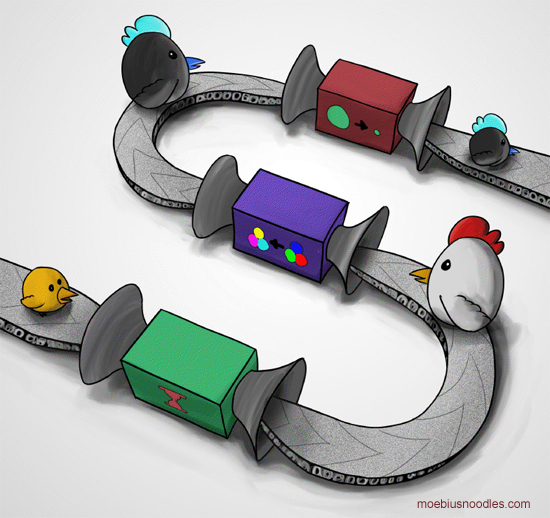
\includegraphics[width=.9\linewidth]{./images/higherorder/ThreeFunctionMachines.jpg}

而 underscore 要么是以对象保持中间数据, 用 chaining
的方式对目标应用各种函数(书上会写这是Flow-Base
programming,但我觉得其实是 Monad,会在下一章中介绍),
要么用函数嵌套函数, 将目标一层层传递下去.

\section{pipe}
\label{sec:orgheadline21}

类似 compose, eweda/ramda 还有一个方法叫 pipe, pipe 的函数执行方向刚好与
compose 相反. 比如 \texttt{pipe(f, g)}, \texttt{f} 会先执行, 然后结果传给 \texttt{g},
是不是让你想起了 bash 的 pipe

\begin{verbatim}
find / | grep porno
\end{verbatim}

实际上就是 \texttt{pipe(find, grep(porno))(/)}

没错,他们都是一个意思. 而且这个函数执行的方向更适合人脑编译(可读)一些.

如果你已经习惯 underscore 的这种写法

\begin{verbatim}
_(data)
  .chain()
  .map(data1,fn1)
  .filter(data2, fn2)
  .value()
\end{verbatim}

那么转换成 pipe 是很容易的一件事情,而且更简单明了易于重用和组合。

\begin{verbatim}
pipe(
  map(fn1),
  filter(fn2)
)(data)
\end{verbatim}
\part{Transducers}
\label{sec:orgheadline31}
通过上一篇\href{./clojure-core.async-essence-in-native-javascript.org}{Clojure风格的JavaScript并发编程}介绍了如何用JavaScript享受到Clojure在并发编程的优势. 我决定
写一系列关于如何用JavaScript玩转Clojure大法的文章. 这回要用JavaScript玩转另一个
Clojure全新的概念 -- \emph{Transducer}.

Transducer 是 Rich Hickey\footnote{Clojure的作者} \href{http://blog.cognitect.com/blog/2014/8/6/transducers-are-coming}{高调宣布} 的在Clojure 1.7 版本加入的又一大法. 在之前的另一个概念
\href{http://clojure.com/blog/2012/05/15/anatomy-of-reducer.html}{Reducer} 却没那么 \textbf{高调}. 在解释transducer之前, 先看看什么是Reducer, 如果能看懂, 再接着看Transducer.

\chapter{Reducer}
\label{sec:orgheadline27}
\index{reducer}
说道reduce这个词, 想必JS Developer大多会用过underscore\footnote{我是故意吧reduce的参数顺序写"反"的, 原来underscore是先消费collection的. 至于为什么要反过来
可以参考\href{http://blog.oyanglul.us/javascript/functional-javascript.html#sec-3-2}{这个解释}}(或类似)的reduce方法, 大概形式是这样
\begin{verbatim}
_.reduce(fn, 0, [1,2,3])
\end{verbatim}
大概意思是初始为0, 应用fn到每一个collection(检测coll)元素上,得到一个新的值.

如果加上map, 比如(我要开始用\href{https://github.com/swannodette/mori}{mori}\footnote{clojurescript作者把clojurescript的一些数据结构和函数编译成javascript, 这样就可以用普通js使用
clojure中的数据结构和函数. document严重过时, 建议看导入的\href{https://github.com/swannodette/mori/blob/master/src/mori.cljs}{源代码}, 以及clojure的文档, 接口和clojure基本一致.} 了)
\begin{verbatim}
reduce(sum, 0, map(inc [1,2,3]))
\end{verbatim}

\begin{quote}
Terminology:
\begin{enumerate}
\item reducing 函数: 用来reduce的函数, 比如sum
\item transform: 变换, 从一个函数变另一个函数
\item xf: xform, transform 函数
\item reducible: 可被reduce的,也就是实现reduce接口的,比如所有的collection
\end{enumerate}
\end{quote}

让我们一步一步分析一下这次reduce到底干了什么
\begin{enumerate}
\item map 函数 inc 到 coll 每一个元素, 得到一个新的 coll \texttt{[2,3,4]}
\item reduce 把新coll的每个元素用sum函数, 得到一个新的值.
\end{enumerate}

好吧这就是reduce了, 用一个reducing函数sum去计算coll得出一个新的值.

来看看更好的解法
\section{transform}
\label{sec:orgheadline24}
\index{xform}
reduce函数需要等待map返回新的coll后才能reduce, 那么可不可以一步直接算出来呢?

假如我们有一个函数xf可以变换reducing函数(上例的sum是reducing函数)的形式, 比如
\begin{verbatim}
xf(reduceFn) -> anotherReduceFn
\end{verbatim}

再假如我们的新map函数可以做这种转换
\begin{verbatim}
map(inc)(sum) -> aShinyNewReduceFn
\end{verbatim}

\begin{quote}
map 函数的简单transform实现可以这样实现,如果你感兴趣的话
\begin{verbatim}
function map(fn){
  return function(reduceFn){
    return function(result, input){
      reduceFn(result, fn(input))
    }
  }
}
\end{verbatim}
\end{quote}

那么我们之前的reduce就可以写成

\begin{verbatim}
reduce(map(inc)(sum),0,[1,2,3])
\end{verbatim}

yeah, 现在只需要一步就reduce出来结果了, reduce应用 \texttt{map(inc)(sum)} 来计算值, 只需要遍历一遍coll

\section{\href{http://clojure.org/reducers}{Reducer}}
\label{sec:orgheadline26}
但是如果我们不想改变map函数的接口, 原始形式的接口还是比较好写好读的
\begin{verbatim}
reduce(sum, 0, map(inc [1,2,3]))
\end{verbatim}
那么需要进一步的抽象, 我把新的map函数叫做rmap好了
\begin{verbatim}
function rmap(fn, coll){
  reducer(coll, map(fn))
}
\end{verbatim}
跟以前接口一样,接收函数和coll,但是返回一个由reducer生成的reducible, 所以就变成了
\begin{verbatim}
reduce(sum, 0, reducer([1,2,3], map(inc)))
\end{verbatim}

等等,怎么做到的\ldots{}你已经消费了coll了, 那reducing函数怎么进来的, reducer怎么知道用sum去reduce呢.


\begin{itemize}
\item Reducible
\label{sec:orgheadline25}
\index{reducible}
答案是, 反转reduce的关系, 原来reduce用sum去计算结果, 现在,我们调用reducible的reduce方法来计算结果

\url{./images/came-out.gif}

如果你还没有被我弄晕的话, 准备好, 又来一个新单词 \emph{reducible}. 也就是可以被reduce的东西.

于是我们需要coll实现reduce方法,这样就成为reducible了.

也就是reduce函数现在应该长这样, 我们暂且叫它 \texttt{rreduce}
\begin{verbatim}
function rreduce(reduceFn, init, reducible){
  reducible(reduceFn, init)
}
\end{verbatim}
那么我们的例子就变成了这样
\begin{verbatim}
reducer([1,2,3], map(inc))(sum, 0)
\end{verbatim}
reducer接收coll和xf, 返回reducible函数. 这一切都是lazy的, 直到rreduce调用第coll行才执行.
\begin{verbatim}
function reducer(coll, xf){
  return function(reduceFn, init){
    return coll.reduce(xf(reduceFn), init)      (coll)
  }
}
\end{verbatim}
\end{itemize}

\chapter{Transducer}
\label{sec:orgheadline28}
\index{transducer}
说了半天Reducer,明明说好的要解释的Transducer呢?

如果你还能follow, 那么现在要开始解释Transducer了

其实你已经见过Transducer了, 再回顾一下之前说的Reducer
\begin{enumerate}
\item 接收一个xf函数和一个coll
\item 用xf转换reducing函数, 并应用到coll
\end{enumerate}

Transducer就是那个xf
\begin{verbatim}
reduce(map(inc)(sum),0,[1,2,3])
\end{verbatim}
也就是这里面的 \texttt{map(inc)}

靠, 就这么简单?

就是这么简单, 前面说了reducer的出现是因为想保持原始reduce的api不便, 那么tranducer则提供了
另外一种reduce api

\begin{verbatim}
transduce(map(inc), sum, 0, [1,2,3])
\end{verbatim}
transduce接收一个transducer,一个reducing function, 一个初始值, 一个coll. 这段代码跟前面干的事情一模一样.

另外牛逼的是transducer跟context完全没有关系, 就是完全与数据解耦开来, 比如我们组装好一个transducer xf

可以用在任何地方
\begin{verbatim}
seq(xf data) //生成一个lazy的序列, 同时lazy transform, 每次取的时候data会被transform
into([], xf data) //把 data transform后放到一个数组里
chan(1, xform) // 当数据经过CSP的channel时被transform
\end{verbatim}


\chapter{Is it Curry?}
\label{sec:orgheadline29}
怎么看着有点像柯里化, 一样么?

当然不是, 柯里化或者部分参数只是部分配置参数, 而transducer是一次多n次转换的组合

比如一个柯里化的map可以
\begin{verbatim}
var mapinc = map(inc)
mapinc([1,2,3])
\end{verbatim}

而不能
\begin{verbatim}
mapinc(sum)
\end{verbatim}
因为map就俩参数, 第一个是函数第二个是data, 如果再给data会错误

但是tranceducer只是转换, 所以只接受reducing函数
\begin{verbatim}
reduce(mapinc(sum), 0, [1,2,3])
// => 9
\end{verbatim}

\chapter{完整例子}
\label{sec:orgheadline30}

\part{Functor}
\label{sec:orgheadline35}

\chapter{Functor}
\label{sec:orgheadline32}

Functor 是 可以被 map over 的类型. 什么叫 map over\ldots{}

比如 list 就可以说是可以被map over\ldots{} 那么是不是可枚举类型?

不是的, 来看看 Haskell 中如何解释(其实所有函数式的概念可能用 haskell
是最能说明问题的了).

\begin{verbatim}
ghci > :t fmap
fmap :: (a -> b) -> fa -> f b
\end{verbatim}

\texttt{fmap} 又是什么东西, fmap 是 map over Functor 的函数.
这个函数只干一个事情, 可能通过前面解释的一点点
Haskell功夫,你可能能翻译 \texttt{(a -> b) -> fa -> f b} 了把. 给定一个从 \texttt{a} 到 \texttt{b}
的映射函数, 再给定一个 a 的 Functor, 返回一个 b 的 Functor.

虽然个个字都认识, 但怎么就不知道啥意思.

如果我再说一个新词, 你是不是会疯掉了-- Lift.

好吧, 把他们都串起来, 你就明白了. 
\begin{enumerate}
\item 平常我们可以把 \texttt{a} 到 \texttt{b} 的映射可以叫做 map, 映射的方式就是函数了.
\item 那么类似的对于函数或者其他可以做这种 map 操作的类型或一种计算方式, 叫做 Functor.
\item 而这种 map 就叫做 fmap, 给定 a 集合到 b 集合的映射方式(也就是一个函数), 就能找到 对 a 的一种计算(computation, 任何可变换的类型, 这就是 Functor) 的变换 -- 对 b 的对应计算方式.
\item 如果该计算是一个函数, 那么这个操作叫做 lifting. 非常形象的, 根据 a 到 b 的映射 lift(举) 到另一个层面上.
\end{enumerate}

\url{http://learnyouahaskell-zh-tw.csie.org/img/lifter.png}

虽然 lifting 很形象, 但是还是越说越抽象了, 来举个栗子. 
\chapter{举个栗子🌰}
\label{sec:orgheadline33}
\begin{quote}
注意我们还没有实现 Functor, 因此下面的栗子还不能运行在你的
console.
\end{quote}

前面说了, Functor 可以是数组, 因为数组可以被 map over

\begin{verbatim}
var plus1 = n => n+1;
fmap(plus1, [2, 4, 6, 8])// => [3,5,7,9]
\end{verbatim}

这里,数组 Array 就是 Functor 类型, 而 fmap 把 2 -> 3 的映射方式对 Array
[2,4,6,8] 进行了变换, 得到 [3,5,7,9]. 这跟数组的 map 方法一样,
比较好理解.

再试试换一种 Functor 类型, 试试函数

\begin{verbatim}
var times2 = m => m*2;
fmap(plus1, times2) // => function(){}
fmap(plus1, times2)(3) // => 7 (3*2+1)
\end{verbatim}

看到 fmap 返回的是一个函数, 因为你 map over 的是一个函数 \texttt{times2}. 还记得
\texttt{(a -> b) -> f a -> f b} 的公式么, 因为现在的 Functor 为 Function 类型,
我们可以把=f=替换成函数也就是 x 到 y 的映射, 因此我们可以将该公式替换为

\begin{verbatim}
(a -> b) -> (x -> a) -> (x -> b)
\end{verbatim}

再用我们具体的函数 plus1 替换进去

\begin{verbatim}
(n->n*2) -> plus1(n) -> plus1(n*2)
\end{verbatim}

也就是说, 这个 fmap 会把函数 times2 应用到 plus1 的任何结果上.

这不就是函数组合吗 \texttt{plus1(times2(3))}, 确实是的. 但这只是 Functor
的冰山一角, dan在来看看别的Functor

Functor 还可以是别的东西\ldots{}比如

\begin{verbatim}
fmap(plus1, Either(10, 20))
\end{verbatim}

Either也是 Functor, 慢着, Either 是什么类型, 好吧,在解释 Either 之前,
我们先忍一忍, 来先看看 JavaScript 中怎么实现以及使用一个 Functor.

\chapter{Functor in JavaScript}
\label{sec:orgheadline34}

首先, 我们用定义一个确定 Functor 类型的函数, 如果没有注册的类型抛出异常.

\begin{verbatim}
var types = function(obj) {
  throw new TypeError("fmap called on unregistered type: " + obj);
};
\end{verbatim}

然后实现注册 Functor 的函数.

\begin{verbatim}
 Functor = function(type, defs) {
        var oldTypes = types;
        types = (obj) => {
            if (type.prototype.isPrototypeOf(obj)) {
                return defs; // 这是递归的出口, 判断类型, 确定 fmap 的 Functor 实例属于注册的哪一个 Functor
            }
            return oldTypes(obj); //不断递归寻找 types, 这个效率会很低, 因为调用栈上好多闭包, 每个闭包都保持着 type 和 defs
        }
};
\end{verbatim}

这样可以用 Functor 函数注册一个新的 Functor 类型并定义它自己的 fmap
方法(还记得前面说的 Functor 只有一个方法吗). 比如我们要把 Array 变成
Functor

\begin{verbatim}
Functor(Array, {
    fmap: (fn, array) => {
        arr.map(x => fn(x))
    }
})
\end{verbatim}

好像快要完成的样子. 现在还差 fmap Functor 类型函数了.
这个函数干两件事情, 找到实例属于哪个 Functor 类型, 并调用他的 fmap 方法.

\begin{verbatim}
fmap = eweda.curry((fn, obj) => {
    return types(obj).fmap(f, obj)
})
\end{verbatim}

同样的, 我们很快可以把 Function 也变成 Functor

\begin{verbatim}
Functor(Function, {
    fmap: (f, g) => {
        return eweda.compose(f, g);
}})
\end{verbatim}

还记得前面说 fmap 函数像函数组合吗, 呵呵, 我们这里就按函数组合实现.

\rule{\linewidth}{0.5pt}

来总结一下 fmap 和 Functor 到底是什么, fmap 可以将函数应用到 Functor 上,
Functor 可以看做是容器或者是带 context 的值. 也就是说如果我们想变换 x
的值, 直接给一个函数映射 \texttt{x=> x*2} 即可. 如果我想变换一个数组, 一个函数,
或者 Either 这种带有 context 的或者说容器里面的值,
总不能直接把这些容器直接给函数吧,这时就需要 fmap
将函数的映射关系应用到容器里面的值.
其实就是打开,调一下函数,完了再包好。

好吧, 通过如何实现和使用一个简单的 Functor, 概念上已经估计可以理解了,
我们回过头来看看 Either 是神马玩意.

\href{http://jsbin.com/xezun/1/embed?js,console}{完整代码}
\part{Monad}
\label{sec:orgheadline42}

这个概念好难解释, 你可以理解为一个 Lazy 或者是状态未知的盒子.
听起来像是\href{http://zh.wikipedia.org/wiki/\%E8\%96\%9B\%E5\%AE\%9A\%E8\%B0\%94\%E7\%8C\%AB}{薛定谔猫}(估计点进去你会更晕了).
其实就是的, 在你打开这个盒子之前, 你是不知道里面的猫处在那种状态.

Monad 这个黑盒子, 里面到底卖的神马药,我们要打开喝了才知道.

等等, 不是说好要解释 Either 的吗, 嗯嗯, 这里就是在解释 Either. 上节说
Either 是一个 Functor, 可以被 fmap over. 怎么这里又说道黑盒子了? 好吧,
Monad 其实也是 Functor. 还记得我说的 Functor 其实是一个带 context
的盒子吗. 而 fmap 使得往盒子里应用函数变换成为了可能.

\chapter{Either}
\label{sec:orgheadline36}

先来看看 Either 这种类型会干什么事情.
\href{http://hackage.haskell.org/package/base-4.7.0.0/docs/Data-Either.html#t:Either}{Either}表示要不是左边就是右边的值,
因此我们可以用它来表示薛定谔猫, 要不是活着, 要不死了. Either 还有个方法:
either

\begin{verbatim}
(a -> c) -> (b -> c) -> Either a b -> c
\end{verbatim}

想必你已经对箭头 \texttt{->} 非常熟了吧.如果前面几章你都跳过了,我再翻译下好了.
这里表示接收函数 \texttt{a->c} 和函数 \texttt{b->c}, 再接收一个 Either, 如果 Either
的值在左边,则使用函数映射 \texttt{a->c}, 若值在右边,则应用第二个函数映射 \texttt{b->c}.

作为 Monad, 它还必须具备一个方法 '>>='(这个符号好眼熟的说, 看看 haskell
的 logo, 你就知道 Monad 是有多重要), 也就是 bind 方法.

\url{http://www.haskell.org/wikistatic/haskellwiki_logo.png}

bind 方法的意思很简单, 就是给这个盒子加一个操作,
比如往盒子在加放射性原子,如果猫活着,就是绿巨猫,
如果猫是死的,那就是绿巨死猫.

\begin{verbatim}
Left("cat").bind(cat => Right('hulk'+cat))
// => Left "hulkcat"
Right("deadcat").bind(cat => Left('hulk' + cat))
// => Right "hulkdeadcat"
\end{verbatim}

这有个毛用啊. 表急\ldots{} 来看个经典例子 

\chapter{走钢索}
\label{sec:orgheadline39}

皮尔斯决定要辞掉他的工作改行试着走钢索。他对走钢索蛮在行的,不过仍有个小问题。就是鸟会停在他拿的平衡竿上。他们会飞过来停一小会儿,然后再飞走。这样的情况在两边的鸟的数量一样时并不是个太大的问题。但有时候,所有的鸟都会想要停在同一边,皮尔斯就失去了平衡,就会让他从钢索上掉下去。

\url{http://learnyouahaskell-zh-tw.csie.org/img/pierre.png}

我们这边假设两边的鸟差异在三个之内的时候,皮尔斯仍能保持平衡。

\section{一般解法}
\label{sec:orgheadline37}

首先看看不用 Monad 怎么解

\begin{verbatim}
eweda.installTo(this);
var landLeft = eweda.curry(function(n, pole){
    return [pole[0]+n, pole[1]];
});
var landRight = eweda.curry(function(n, pole){
    return eweda.reverse(landLeft(n, eweda.reverse(pole)));
});
var result = eweda.pipe(landLeft(1), landRight(1), landLeft(2))([0,0]);
console.log(result);
// => [3, 1]
\end{verbatim}

还差一个判断皮尔斯是否掉下来的操作.

\begin{verbatim}
var landLeft = eweda.curry(function(n, pole){
    if(pole==='dead') return pole;
    if(Math.abs(pole[0]-pole[1]) > 3)
      return 'dead';
    return [pole[0]+n, pole[1]];
});
var landRight = eweda.curry(function(n, pole){
    if(pole==='dead') return pole;
    return eweda.reverse(landLeft(n, eweda.reverse(pole)));
});
var result = eweda.pipe(landLeft(10), landRight(1), landRight(8))([0,0]);
console.log(result);
// => dead
\end{verbatim}

\href{http://jsbin.com/pozim/8/watch?js,console,output}{完整代码}

\rule{\linewidth}{0.5pt}

\section{现在来试试用 Either}
\label{sec:orgheadline38}

我们先把皮尔斯放进 Either 盒子里, 这样皮尔斯的状态只有打开 Either
才能看见. 假设 Either Right 是活着, Left 的话皮尔斯挂了.

\begin{verbatim}
var land = eweda.curry(function(lr, n, pole){
    pole[lr] = pole[lr] + n;
    if(Math.abs(pole[0]-pole[1]) > 3) {
      return new Left("dead when land " + n + " became " + pole);
    }
    return new Right(pole);
});

var landLeft = land(0)
var landRight = land(1);
\end{verbatim}

现在落鸟后会返回一个 Either, 要不活着, 要不挂了.
打开盒子的函数可以是这样的

\begin{verbatim}
var stillAlive = function(x){
    console.log(x)
}
var dead = function(x){
    console.log('皮尔斯' + x);
}
either(dead, stillAlive, landLeft(2, [0,0]))
\end{verbatim}

好吧, 好像有一点点像了, 但是这只落了一次鸟, 如果我要落好几次呢.
这就需要实现 Either 的 >>= bind 方法了, 如果你还记得前面实现的 Functor,
这里非常像 :

\begin{verbatim}
var Monad = function(type, defs) {
  for (name in defs){
    type.prototype[name] = defs[name];
  }
  return type;
};
function Left(value){
  this.value = value
}
function Right(value){
  this.value=value;
}

Monad(Right, {
  bind:function(fn){
    return fn(this.value)
  }
})

Monad(Left, {
  bind: function(fn){
    return this;
  }
})
\end{verbatim}

哦, 对了, either:

\begin{verbatim}
either = function(left, right, either){
    if(either.constructor.name === 'Right')
        return right(either.value)
    else
        return left(either.value)
}
\end{verbatim}

我们来试试工作不工作.

\begin{verbatim}
var walkInLine = new Right([0,0]);
eitherDeadOrNot = walkInLine.bind(landLeft(2))
    .bind(landRight(5))
either(dead, stillAlive, eitherDeadOrNot)
// => [2,5]
eitherDeadOrNot = walkInLine.bind(landLeft(2))
  .bind(landRight(5))
  .bind(landLeft(3))
  .bind(landLeft(10)
  .bind(landRight(10)))

either(dead, stillAlive, eitherDeadOrNot)
// => "皮尔斯dead when land 10 became 15,5"
\end{verbatim}

\href{http://jsbin.com/giyig/3/watch}{完整代码}

\chapter{到底有什么用呢, Monad}
\label{sec:orgheadline40}

我们来总结下两种做法有什么区别:

\begin{enumerate}
\item 一般做法每次都会检查查尔斯挂了没挂, 也就是重复获得之前操作的 context
\item Monad 不对异常做处理, 只是不停地往盒子里加操作. 你可以看到对错误的处理推到了最后取值的 either.
\item Monad 互相传递的只是盒子, 而一般写法会把异常往下传如 \texttt{dead}, 这样导致后面的操作都得先判断这个异常.
\end{enumerate}

\begin{quote}
由于是用 JavaScript, pole 不限定类型,
所以这里单纯的用字符串代表 pole 的异常状态. 但如果换成强类型的 Java,
可能实现就没这么简单了.
\end{quote}

看来已经优势已经逐步明显了呢, Monad 里面保留了值的 context,
也就是我们对这个 Monad 可以集中在单独的本次如何操作value, 而不用关心
context.

\begin{quote}
还有一个 Monad 叫做 Maybe, 实际上皮尔斯的🌰用 Maybe 更为合适, 因为
Maybe 有两种状态, 一种是有值 Just, 一种是没东西 Nothing,
可以自己实现试试.
\end{quote}

\chapter{Monad 在 JavaScript 中的应用}
\label{sec:orgheadline41}

你知道 ES6有个新的 类型
\href{https://developer.mozilla.org/en-US/docs/Web/JavaScript/Reference/Global_Objects/Promise#Browser_compatibility}{Promise}
吗, 如果不知道, 想必也听过 jQuery 的 \texttt{\$.ajax} 吧, 但如果你没听过 promise,
说明你没有认真看过他的返回值:

\begin{verbatim}
var aPromise = $.ajax({
    url: "https://api.github.com/users/jcouyang/gists"
    dataType: 'jsonp'
    })
aPromise /***
=> Object { state: .Deferred/r.state(),
    always: .Deferred/r.always(),
    then: .Deferred/r.then(),
    promise: .Deferred/r.promise(),
    pipe: .Deferred/r.then(),
    done: b.Callbacks/p.add(),
    fail: b.Callbacks/p.add(),
    progress: b.Callbacks/p.add() }
***/
\end{verbatim}

我们看到返回了好多 \texttt{Deferred} 类型的玩意, 我们来试试这玩意有什么用

\begin{verbatim}
anotherPromise = aPromise.then(_ => _.data.forEach(y=> console.log(y.description)))
/* =>
Object { state: .Deferred/r.state(),
    always: .Deferred/r.always(),
    then: .Deferred/r.then(),
    promise: .Deferred/r.promise(),
    pipe: .Deferred/r.then(),
    done: b.Callbacks/p.add(),
    fail: b.Callbacks/p.add(),
    progress: b.Callbacks/p.add() }

"connect cisco anyconnect in terminal"
"为什么要柯里化(curry)"
"批量获取人人影视下载链接"
......
*/
\end{verbatim}

看见没有, 他又返回了同样一个东西, 而且传给 then
的函数可以操作这个对象里面的值. 这个对象其实就是 Promise 了.
为什么说这是 Monad 呢, 来试试再写一次 \texttt{走钢丝}:

\begin{quote}
这里我们用的是 ES6 的 Promise, 而不用 jQuery Defered, 记得用 firefox
哦. 另外 eweda 可以这样装
\end{quote}

\begin{verbatim}
var ewd = document.createElement('script'); dsq.type = 'text/javascript'; dsq.async = true;
            ewd.src = 'https://rawgit.com/CrossEye/eweda/master/eweda.js';
(document.getElementsByTagName('head')[0] || document.getElementsByTagName('body')[0]).appendChild(ewd);
eweda.installTo(this);
\end{verbatim}

\begin{verbatim}
var land = eweda.curry(function(lr, n, pole){
    pole[lr] = pole[lr] + n;
    if(Math.abs(pole[0]-pole[1]) > 3) {
      return new Promise((resovle,reject)=>reject("dead when land " + n + " became " + pole));
    }
    return new Promise((resolve,reject)=>resolve(pole));
});

var landLeft = land(0)
var landRight = land(1);

Promise.all([0,0])
.then(landLeft(2), _=>_)
.then(landRight(3), _=>_) // => Array [ 2, 3 ]
.then(landLeft(10), _=>_)
.then(landRight(10), _=>_)
.then(_=>console.log(_),_=>console.log(_))
// => "dead when land 10 became 12,3"
\end{verbatim}

这下是不承认 Promise 就是 Monad 了. 原来我们早已在使用这个神秘的 Monad,
再想想 Promise,也没有那么抽象和神秘了.
\end{document}
